\chapter{Equilíbrios de oxirredução e a equação de Nernst}\label{ch:b1:nernst}

Coloque uma lâmina de zinco em uma solução de sulfato de zinco e uma
lâmina de cobre em uma solução de sulfato de cobre(II), ligue as duas
soluções por um tubo com solução salina e os dois metais por um fio que
passa por um diodo emissor de luz: o diodo acende. A reação do zinco com
os íons cobre, que em um único béquer apenas aquece a solução, agora
impulsiona elétrons através de um fio. Uma pilha é esse arranjo,
embalado; um pHmetro e um eletrodo de cloreto são seus primos de medida.
Este capítulo torna quantitativa a troca de elétrons: os \omterm{def:b1:nernst:oxidation-number}{números de
oxidação} para contar os elétrons, os \omterm{def:b1:nernst:electrode-potential}{potenciais de eletrodo} para
ordenar os pares e a \omterm{thm:b1:nernst:nernst}{equação de Nernst} para acompanhá-los em função da
concentração.

\begin{recall}
O volume escolar (anos 11 e 12) definiu \omterm{def:b1:nernst:couple}{oxidantes} e \omterm{def:b1:nernst:couple}{redutores}, escreveu
\omterm{def:b1:nernst:couple}{semirreações}, montou pilhas com dois metais e duas soluções e leu a
pilha zinco--cobre como uma bateria. O \omterm{def:b1:extent-q-and-k:quotient}{quociente de reação} e a constante
de equilíbrio são os do \cref{ch:b1:extent-q-and-k}; as \omterm{def:b1:extent-q-and-k:activity}{atividades} são
$c/c^\circ$ para os solutos e $p/p^\circ$ para os gases, 1 para os
sólidos e líquidos puros.
\end{recall}

\section{Números de oxidação e pares}

\begin{definition}[Oxidante, redutor, par redox, semirreação]\label{def:b1:nernst:couple}
Um \emph{oxidante}\index{oxidante} é uma espécie capaz de ganhar
elétrons; um \emph{redutor}\index{redutor}, uma espécie capaz de
cedê-los. Um oxidante Ox e o redutor Red em que ele se transforma formam
um \emph{par redox}\index{par redox} Ox/Red, descrito por sua
\emph{semirreação}\index{semirreacao@semirreação}
$\alpha\,\mathrm{Ox} + n\,\mathrm{e^-} \rightleftharpoons
\beta\,\mathrm{Red}$, balanceada em átomos com \ce{H2O} e \ce{H+} quando
necessário e em carga com os elétrons.
\end{definition}

Uma reação de oxirredução é a troca de elétrons entre dois pares: o
\omterm{def:b1:nernst:couple}{oxidante} de um é reduzido enquanto o \omterm{def:b1:nernst:couple}{redutor} do outro é oxidado, e os
elétrons se cancelam. Para contá-los em uma espécie complicada,
atribui-se a cada átomo um \omterm{def:b1:nernst:oxidation-number}{número de oxidação}.

\begin{definition}[Número de oxidação]\label{def:b1:nernst:oxidation-number}
O \emph{número de oxidação}\index{numero de oxidacao@número de oxidação} de um átomo em uma
espécie é a carga que ele teria se todas as ligações fossem rompidas
entregando os dois elétrons de ligação ao átomo mais eletronegativo
(compartilhados igualmente entre dois átomos idênticos). Ele é escrito
em algarismos romanos: ferro(III), \ce{Mn^{+VII}} no íon permanganato.
\end{definition}

\begin{proposition}[Regras dos números de oxidação]\label{prop:b1:nernst:on-rules}
\begin{enumerate}
  \item Um átomo em uma substância simples tem \omterm{def:b1:nernst:oxidation-number}{número de oxidação} 0; um
        íon monoatômico tem a sua carga.
  \item Os \omterm{def:b1:nernst:oxidation-number}{números de oxidação} dos átomos de uma espécie somam a sua
        carga.
  \item O hidrogênio é $+$I (exceto nos hidretos metálicos, $-$I); o
        oxigênio é $-$II (exceto nos peróxidos, $-$I, e ligado ao flúor);
        o flúor é $-$I.
  \item Em uma \omterm{def:b1:nernst:couple}{semirreação}, o número de elétrons é igual à variação do
        \omterm{def:b1:nernst:oxidation-number}{número de oxidação} do elemento que muda, vezes o número de seus
        átomos.
\end{enumerate}
\end{proposition}

\begin{proof}
1 e 2: romper todas as ligações conserva a carga, e entre átomos
idênticos nada é transferido. 3: o hidrogênio é menos eletronegativo que
todos os não metais aos quais se liga (\cref{ch:b1:periodicity}) e mais
que os metais alcalinos; o oxigênio é mais eletronegativo que todos os
elementos, exceto o flúor, e em \ce{O-O} o par compartilhado é dividido.
4: H e O mantêm seus números, de modo que os únicos átomos cuja carga
fictícia muda são os do elemento considerado, e os elétrons aparecem na
\omterm{def:b1:nernst:couple}{semirreação} exatamente para compensar essa variação de carga.
\end{proof}

\begin{method}[Números de oxidação de uma espécie]\label{met:b1:nernst:oxidation-numbers}
Dê a H, O, F e aos íons seus números usuais; o número do átomo restante
decorre da regra 2. Em \ce{MnO4-}: $x + 4(-2) = -1$, $x = +7$. Em
\ce{Cr2O7^2-}: $2x - 14 = -2$, $x = +6$. Em \ce{S4O6^2-}, a média é
$+2.5$; a \omterm{def:b1:lewis-resonance-vsepr:lewis}{estrutura de Lewis} mostra dois tipos de enxofre.
\end{method}

\begin{method}[Balancear uma semirreação]\label{met:b1:nernst:balance-by-on}
\begin{enumerate}
  \item Balanceie o elemento cujo \omterm{def:b1:nernst:oxidation-number}{número de oxidação} muda.
  \item Acrescente os elétrons: a variação do \omterm{def:b1:nernst:oxidation-number}{número de oxidação} vezes o
        número de átomos.
  \item Balanceie a carga com \ce{H+} (solução ácida) ou \ce{OH-}
        (solução básica).
  \item Balanceie o hidrogênio e o oxigênio com \ce{H2O}; verifique o
        oxigênio por último.
\end{enumerate}
Para o íon permanganato em meio ácido: Mn passa de $+$VII a $+$II, logo 5
elétrons; a carga à esquerda é $-1 - 5 = -6$ e à direita $+2$, logo
$8\,\ce{H+}$; depois $4\,\ce{H2O}$:
\ce{MnO4- + 8H+ + 5e- -> Mn^2+ + 4H2O}.
\end{method}

\section{Pilhas eletroquímicas}

\begin{definition}[Pilha eletroquímica]\label{def:b1:nernst:cell}
Uma \emph{pilha eletroquímica}\index{pilha eletroquimica@pilha eletroquímica} é formada por duas
\emph{meias-pilhas}\index{meia-pilha}, cada uma constituída por um par e um
condutor eletrônico, o eletrodo, ligadas por um condutor iônico, muitas
vezes uma \emph{ponte salina}\index{ponte salina} (um gel ou um tubo com
um sal inerte concentrado, como o nitrato de potássio). O eletrodo em
que ocorre a oxidação é o \emph{ânodo}\index{anodo@ânodo}; aquele em que
ocorre a redução, o \emph{cátodo}\index{catodo@cátodo}. A \emph{tensão da
pilha}\index{tensao da pilha@tensão da pilha} é a diferença de potencial elétrico
entre os dois eletrodos, polo positivo menos polo negativo, medida
quando nenhuma corrente circula.
\end{definition}

\begin{omfigure}
\begin{tikzpicture}[font=\small, >={Stealth}]
  \pic at (0,0) {beaker={0.7}{omDef!14}};
  \pic at (3.6,0) {beaker={0.7}{omDef!32}};
  \pic at (-0.3,0.25) {electrode={black!35}};
  \pic at (3.9,0.25) {electrode={orange!70!brown}};
  \pic at (0.35,0.55) {saltbridge={2.9}};
  \pic (m) at (1.8,4.3) {meter={V}};
  \draw[thick] (-0.15,2.65) |- (m-a);
  \draw[thick] (4.05,2.65) |- (m-b);
  \node[anchor=east] at (-0.95,1.0) {\ce{Zn}};
  \node[anchor=west] at (4.45,1.0) {\ce{Cu}};
  \node at (0.25,-0.35) {\ce{Zn^2+}, \ce{SO4^2-}};
  \node at (3.6,-0.35) {\ce{Cu^2+}, \ce{SO4^2-}};
  \draw[->, omProp, thick] (-0.15,3.35) -- (0.8,3.35) node[above, midway] {$\mathrm{e^-}$};
  \draw[->, omProp, thick] (2.8,3.35) -- (3.75,3.35) node[above, midway] {$\mathrm{e^-}$};
  \node[anchor=east] at (-0.9,2.3) {$-$ ânodo};
  \node[anchor=west] at (4.6,2.3) {cátodo $+$};
  \node[font=\scriptsize, align=center] at (1.8,2.75) {ponte salina\\ \ce{K+} $\rightarrow$ \quad $\leftarrow$ \ce{NO3-}};
  \node[font=\scriptsize] at (-0.1,-0.8) {\ce{Zn -> Zn^2+ + 2e-}};
  \node[font=\scriptsize] at (3.7,-0.8) {\ce{Cu^2+ + 2e- -> Cu}};
\end{tikzpicture}

{\small A pilha zinco--cobre (pilha de Daniell). O zinco é oxidado no
\omterm{def:b1:nernst:cell}{ânodo}, o polo negativo; os íons cobre são reduzidos no \omterm{def:b1:nernst:cell}{cátodo}, o polo
positivo. Os elétrons circulam pelo circuito externo do zinco para o
cobre; na \omterm{def:b1:nernst:cell}{ponte salina}, os cátions migram em direção ao \omterm{def:b1:nernst:cell}{cátodo} e os
ânions em direção ao \omterm{def:b1:nernst:cell}{ânodo}, mantendo cada solução neutra.}
\end{omfigure}

Uma pilha é escrita em uma linha, com o \omterm{def:b1:nernst:cell}{ânodo} à esquerda: \ce{Zn} $|$ \ce{Zn^2+}
$\|$ \ce{Cu^2+} $|$ \ce{Cu}, barras simples para as interfaces, barra dupla
para a \omterm{def:b1:nernst:cell}{ponte salina}. Com todas as concentrações a \qty{1}{mol/L}, sua
tensão é de \qty{1.10}{V}. A reação que ocorre quando a pilha fornece
corrente, \ce{Zn + Cu^2+ -> Zn^2+ + Cu}, é a que aconteceria em um único
béquer; separar as \omterm{def:b1:nernst:cell}{meias-pilhas} obriga os elétrons a passar pelo fio,
onde podem realizar trabalho.

\section{Potenciais de eletrodo}

Uma tensão é uma diferença: só se podem medir diferenças entre duas
\omterm{def:b1:nernst:cell}{meias-pilhas}. Escolhe-se, portanto, de uma vez por todas uma \omterm{def:b1:nernst:cell}{meia-pilha}
de referência.

\begin{definition}[Potencial de eletrodo, potencial padrão]\label{def:b1:nernst:electrode-potential}
O \emph{eletrodo padrão de hidrogênio}\index{eletrodo padrao de hidrogenio@eletrodo padrão de hidrogênio}
é um eletrodo de platina em contato com gás hidrogênio a \qty{1}{bar} e
com uma solução ideal de \ce{H+} de \omterm{def:b1:extent-q-and-k:activity}{atividade} 1. O \emph{potencial de
eletrodo}\index{potencial de eletrodo} $E$ de uma \omterm{def:b1:nernst:cell}{meia-pilha} é a \omterm{def:b1:nernst:cell}{tensão
da pilha} formada com o eletrodo padrão de hidrogênio à esquerda:
$E = V_{\text{meia-pilha}} - V_{\text{EPH}}$. Quando todas as espécies
do par têm \omterm{def:b1:extent-q-and-k:activity}{atividade} 1, ele é o \emph{potencial padrão}\index{potencial padrao@potencial padrão}
$E^\circ$ do par, uma constante a uma dada temperatura.
\end{definition}

\begin{omfigure}
\begin{tikzpicture}[font=\small, >={Stealth}]
  \pic at (0,0) {beaker={0.72}{omDef!14}};
  % glass jacket, open at the bottom, with the gas inlet on the right
  \draw[om glass] (-0.32,0.35) -- (-0.32,3.0) -- (0.32,3.0) -- (0.32,2.55)
    -- (0.95,2.55) (0.32,2.35) -- (0.95,2.35) (0.32,2.35) -- (0.32,0.35);
  \draw[thick] (0,0.9) -- (0,3.45);
  \fill[black!60] (-0.16,0.5) rectangle (0.16,0.9);
  \foreach \x/\y in {0.45/0.45, 0.55/0.75, 0.48/1.05, -0.45/0.5, -0.52/0.85}
    \draw[omDef!70] (\x,\y) circle (0.055);
  \draw[->] (1.9,2.45) node[right] {\ce{H2}, \qty{1}{bar}} -- (1.0,2.45);
  \draw (0.12,0.7) -- (1.5,0.2) node[right] {platina platinizada};
  \draw (-0.6,1.1) -- (-1.4,1.6) node[left] {\ce{H+}, atividade 1};
  \node[anchor=west] at (0.05,3.45) {para o circuito};
\end{tikzpicture}

{\small O \omterm{def:b1:nernst:electrode-potential}{eletrodo padrão de hidrogênio}: o gás hidrogênio borbulha sobre
uma placa de platina recoberta de platina finamente dividida, mergulhada
em uma solução na qual \ce{H+} tem \omterm{def:b1:extent-q-and-k:activity}{atividade} 1. Seu par é
\ce{H+}/\ce{H2}, de potencial 0 por convenção.}
\end{omfigure}

O eletrodo de hidrogênio é incômodo de usar; os laboratórios medem em
relação a uma \omterm{def:b1:nernst:cell}{meia-pilha} mais prática, cujo potencial é conhecido.

\begin{definition}[Eletrodo de referência]\label{def:b1:nernst:reference-electrode}
Um \emph{eletrodo de referência}\index{eletrodo de referencia@eletrodo de referência} é uma
\omterm{def:b1:nernst:cell}{meia-pilha} cujo potencial é fixo e conhecido: o eletrodo de
prata--cloreto de prata (um fio de prata recoberto de cloreto de prata
em uma solução de cloreto de concentração fixa) ou o eletrodo de
calomelano (mercúrio em contato com \ce{Hg2Cl2} e uma solução de
cloreto).
\end{definition}

A tabela abaixo dá os \omterm{def:b1:nernst:electrode-potential}{potenciais padrão} usados neste volume; a escala
vertical da próxima seção mostra os mais comuns.

\begin{omfigure}
\begin{tabular}{lr@{\qquad}lr}
\hline
par & $E^\circ$ (V) & par & $E^\circ$ (V) \\
\hline
\ce{Li+}/\ce{Li} & $-3.04$ & \ce{Cu^2+}/\ce{Cu} & 0.34 \\
\ce{K+}/\ce{K} & $-2.94$ & $[\ce{Fe(CN)6}]^{3-}$/$[\ce{Fe(CN)6}]^{4-}$ & 0.36 \\
\ce{Na+}/\ce{Na} & $-2.71$ & \ce{Cu+}/\ce{Cu} & 0.52 \\
\ce{Mg^2+}/\ce{Mg} & $-2.36$ & \ce{I2}/\ce{I-} & 0.53 \\
\ce{Al^3+}/\ce{Al} & $-1.68$ & \ce{O2}/\ce{H2O2} & 0.69 \\
\ce{Zn^2+}/\ce{Zn} & $-0.76$ & \ce{Fe^3+}/\ce{Fe^2+} & 0.77 \\
\ce{Fe^2+}/\ce{Fe} & $-0.41$ & \ce{Hg2^2+}/\ce{Hg} & 0.80 \\
\ce{Ni^2+}/\ce{Ni} & $-0.24$ & \ce{Ag+}/\ce{Ag} & 0.80 \\
\ce{Pb^2+}/\ce{Pb} & $-0.13$ & \ce{Br2}/\ce{Br-} & 1.08 \\
\ce{H+}/\ce{H2} & 0 & \ce{O2}/\ce{H2O} & 1.23 \\
\ce{S4O6^2-}/\ce{S2O3^2-} & 0.02 & \ce{MnO2}/\ce{Mn^2+} & 1.23 \\
\ce{Cu^2+}/\ce{Cu+} & 0.16 & \ce{Cl2}/\ce{Cl-} & 1.36 \\
\ce{AgCl}/\ce{Ag} & 0.22 & \ce{PbO2}/\ce{Pb^2+} & 1.46 \\
\ce{Hg2Cl2}/\ce{Hg} & 0.27 & \ce{MnO4-}/\ce{Mn^2+} & 1.51 \\
 & & \ce{HClO}/\ce{Cl2} & 1.63 \\
 & & \ce{H2O2}/\ce{H2O} & 1.76 \\
\hline
\end{tabular}

\smallskip
{\small \omterm{def:b1:nernst:electrode-potential}{Potenciais padrão} a \qty{25}{\celsius}, calculados a partir das
energias de Gibbs padrão de formação tabeladas das espécies de cada par.
Eles podem diferir em alguns centésimos de volt de outras compilações.}
% ledger: dfg:Li+_ao, dfg:K+_ao, dfg:Na+_ao, dfg:Mg2+_ao, dfg:Al3+_ao, dfg:Zn2+_ao, dfg:Fe2+_ao, dfg:Ni2+_ao, dfg:Pb2+_ao (computed in figdata/bachelor-1/standard-potentials.py)
% ledger: dfg:S4O62-_ao, dfg:S2O32-_ao, dfg:Cu2+_ao, dfg:Cu+_ao, dfg:AgCl_cr, dfg:Cl-_ao, dfg:Hg2Cl2_cr, dfg:Fe_CN63-_ao, dfg:Fe_CN64-_ao, dfg:I-_ao (same script)
% ledger: dfg:H2O2_ao, dfg:Fe3+_ao, dfg:Hg22+_ao, dfg:Ag+_ao, dfg:Br-_ao, dfg:H2O_l, dfg:MnO2_cr, dfg:Mn2+_ao, dfg:PbO2_cr, dfg:MnO4-_ao, dfg:HClO_ao (same script)
\end{omfigure}

\section{A equação de Nernst}

\begin{theorem}[Equação de Nernst]\label{thm:b1:nernst:nernst}
Para um par $\alpha\,\mathrm{Ox} + n\,\mathrm{e^-} \rightleftharpoons
\beta\,\mathrm{Red}$, com eventualmente outras espécies (\ce{H+}, \ce{H2O},
\ce{Cl-}) de um lado ou do outro, o \omterm{def:b1:nernst:electrode-potential}{potencial de eletrodo} é dado pela
\emph{equação de Nernst}\index{equacao de Nernst@equação de Nernst}
\[
  E = E^\circ + \frac{RT}{nF}\ln\frac{\prod a_{\text{lado ox}}^{\nu}}{\prod
  a_{\text{lado red}}^{\nu}}
  = E^\circ + \frac{0.059}{n}\log\frac{a(\mathrm{Ox})^\alpha\,\cdots}{a(\mathrm{Red})^\beta\,\cdots}
  \quad\text{a \qty{25}{\celsius}},
\]
em que cada \omterm{def:b1:extent-q-and-k:activity}{atividade} leva seu \omterm{def:b1:extent-q-and-k:extent}{número estequiométrico} e o fator
$RT\ln 10/F = \qty{0.059}{V}$ a \qty{298}{K}.
\end{theorem}

\admitted{A \omterm{thm:b1:nernst:nernst}{equação de Nernst} decorre da relação entre a energia de Gibbs
de uma reação e a \omterm{def:b1:nernst:cell}{tensão da pilha}, deduzida no volume do 2.º~ano.}

\begin{example}[Três pares]\label{ex:b1:nernst:examples}
\ce{Cu^2+}/\ce{Cu}: $E = 0.34 + 0.030\log[\ce{Cu^2+}]$ (o cobre metálico
tem \omterm{def:b1:extent-q-and-k:activity}{atividade} 1).
\ce{Fe^3+}/\ce{Fe^2+}: $E = 0.77 + 0.059\log([\ce{Fe^3+}]/[\ce{Fe^2+}])$.
\ce{MnO4-}/\ce{Mn^2+}: $E = 1.51 + \frac{0.059}{5}\log
\frac{[\ce{MnO4-}][\ce{H+}]^8}{[\ce{Mn^2+}]}$; com concentrações iguais de
permanganato e de manganês(II), $E = 1.51 - 0.094\,\mathrm{pH}$: o poder
\omterm{def:b1:nernst:couple}{oxidante} do permanganato diminui quando o pH aumenta.
\end{example}

Uma variação de dez vezes em uma concentração desloca o potencial de
$0.059/n$ volt: algumas dezenas de milivolts. É por isso que uma tensão
medida ao milivolt é uma medida precisa de uma concentração, o princípio
do eletrodo de pH e do eletrodo de cloreto do problema de fim de semana.

\begin{history}[Walther Nernst]
\begin{minipage}[t]{0.22\linewidth}\vspace{0pt}
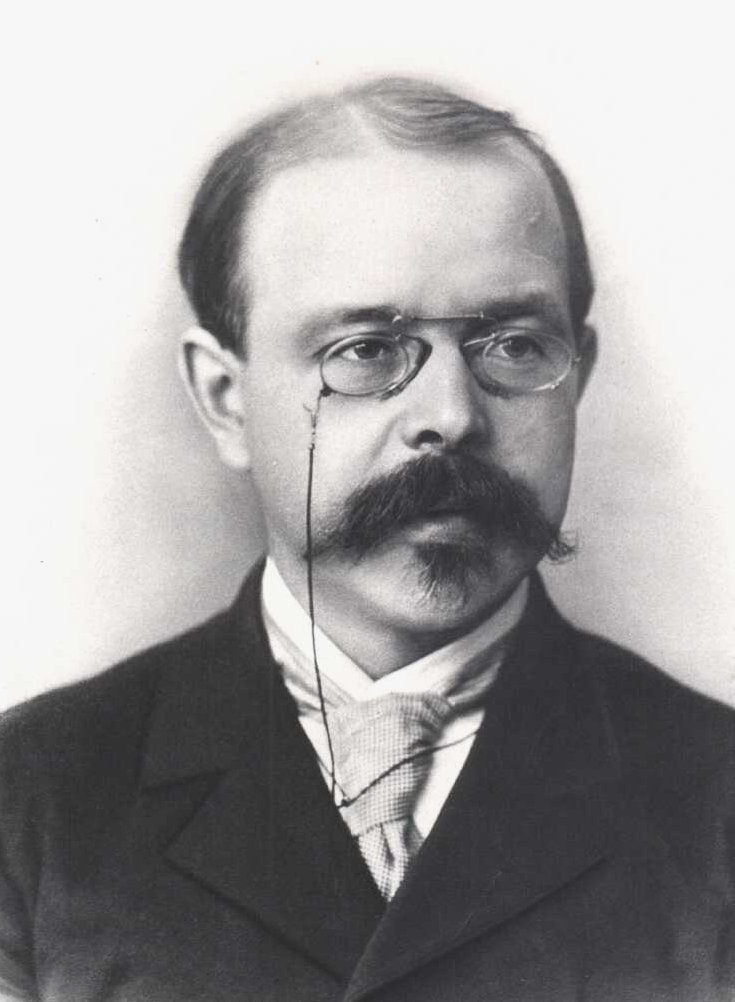
\includegraphics[width=\linewidth]{images/book2/nernst.jpg}
\end{minipage}\hfill
\begin{minipage}[t]{0.74\linewidth}\vspace{0pt}
Walther Nernst (1864--1941), aqui aos vinte e cinco anos, em 1889. A
equação desta seção, que liga a tensão de uma pilha às concentrações de
seus íons, leva o seu nome, assim como um terceiro princípio da
termodinâmica, visto no volume do 2.º~ano. (Fotografia: Smithsonian
Libraries, domínio público, Wikimedia Commons.)
\end{minipage}
\end{history}

\section{Prever reações de oxirredução}

\begin{method}[Prever uma reação de oxirredução]\label{met:b1:nernst:predict-redox}
\begin{enumerate}
  \item Coloque os pares em uma escala vertical de \omterm{def:b1:nernst:electrode-potential}{potenciais padrão},
        os \omterm{def:b1:nernst:couple}{oxidantes} à esquerda, os \omterm{def:b1:nernst:couple}{redutores} à direita.
  \item O \omterm{def:b1:nernst:couple}{oxidante} mais forte presente (maior $E^\circ$) reage com o
        \omterm{def:b1:nernst:couple}{redutor} mais forte presente (menor $E^\circ$): a seta que desce do
        \omterm{def:b1:nernst:couple}{oxidante} até o \omterm{def:b1:nernst:couple}{redutor} e depois sobe até os produtos desenha uma
        letra grega gama, $\gamma$.
  \item A reação é favorecida ($K > 1$) quando o par do \omterm{def:b1:nernst:couple}{oxidante} está
        acima do par do \omterm{def:b1:nernst:couple}{redutor}; na prática, ela é \omterm{def:b1:extent-q-and-k:quantitative}{quantitativa} quando a
        diferença ultrapassa cerca de \qty{0.25}{V} para um elétron
        trocado.
\end{enumerate}
\end{method}

\begin{omfigure}
\begin{tikzpicture}[font=\small, >={Stealth}, y=2.6cm]
  \draw[->, thick] (0,-1.0) -- (0,1.85) node[above] {$E^\circ$ (V)};
  \foreach \e/\o/\r in {-0.76/\ce{Zn^2+}/\ce{Zn}, 0/\ce{H+}/\ce{H2},
      0.34/\ce{Cu^2+}/\ce{Cu}, 0.77/\ce{Fe^3+}/\ce{Fe^2+},
      1.36/\ce{Cl2}/\ce{Cl-}, 1.51/\ce{MnO4-}/\ce{Mn^2+}} {
    \draw (-0.12,\e) -- (0.12,\e);
    \node[anchor=east] at (-0.25,\e) {\o};
    \node[anchor=west] at (0.25,\e) {\r};
    \node[anchor=west, black!55, font=\scriptsize] at (2.0,\e) {\e};
  }
  \node[omProp] at (-1.0,1.85) {oxidantes};
  \node[omDef] at (1.1,1.85) {redutores};
  % the gamma: Cu2+ meets Zn below it on the other side
  \draw[omThm, very thick, ->, rounded corners=4pt] (-1.0,0.28) -- (-1.0,-0.42) -- (0.6,-0.70);
  \draw[omThm, thick, ->] (-0.5,0.40) to[bend left=40] (0.5,0.40);
  \draw[omThm, thick, ->] (0.5,-0.85) to[bend left=40] (-0.5,-0.85);
\end{tikzpicture}

{\small Uma escala de \omterm{def:b1:nernst:electrode-potential}{potenciais padrão}. A regra do gama: o \omterm{def:b1:nernst:couple}{oxidante}
\ce{Cu^2+} reage com o \omterm{def:b1:nernst:couple}{redutor} \ce{Zn}, situado abaixo dele do outro
lado (seta grossa); \ce{Cu^2+} é reduzido a \ce{Cu} (seta curva de
cima) e \ce{Zn} é oxidado a \ce{Zn^2+} (seta curva de baixo). A reação
inversa, de \ce{Cu} com \ce{Zn^2+}, não é favorecida.}
\end{omfigure}

\begin{proposition}[Constante de equilíbrio a partir dos potenciais padrão]\label{prop:b1:nernst:equilibrium-constant}
Para a reação $\mathrm{Ox_1} + \mathrm{Red_2} \rightleftharpoons
\mathrm{Red_1} + \mathrm{Ox_2}$ com troca de $n$ elétrons,
\[
  \log K = \frac{n\,(E^\circ_1 - E^\circ_2)}{0.059}\quad\text{a \qty{25}{\celsius}} .
\]
\end{proposition}

\begin{proof}
No equilíbrio, nenhuma corrente circula em uma pilha construída com os
dois pares: os dois eletrodos têm o mesmo potencial, $E_1 = E_2$.
Escreva a \omterm{thm:b1:nernst:nernst}{equação de Nernst} de cada um com o mesmo $n$: $E^\circ_1 + \frac{0.059}{n}\log
\frac{a(\mathrm{Ox_1})}{a(\mathrm{Red_1})} = E^\circ_2 + \frac{0.059}{n}\log
\frac{a(\mathrm{Ox_2})}{a(\mathrm{Red_2})}$, logo $\frac{n(E^\circ_1 -
E^\circ_2)}{0.059} = \log\frac{a(\mathrm{Red_1})a(\mathrm{Ox_2})}{a(\mathrm{Ox_1})
a(\mathrm{Red_2})} = \log K$, sendo as \omterm{def:b1:extent-q-and-k:activity}{atividades} as do equilíbrio.
\end{proof}

Para a reação de Daniell, $\log K = 2(0.34 + 0.76)/0.059 = 37$: o zinco
reduz completamente os íons cobre. Para \ce{2Fe^3+ + 2I- <=> 2Fe^2+ + I2},
$\log K = 2(0.77 - 0.53)/0.059 = 8.1$. Daí vem o critério do método:
com $n = 1$, uma diferença de \qty{0.25}{V} dá $K = 10^{4.2}$.

\begin{proposition}[Combinação de potenciais]\label{prop:b1:nernst:combined-potentials}
Se os pares $\mathrm{A}/\mathrm{B}$ ($n_1$ elétrons) e
$\mathrm{B}/\mathrm{C}$ ($n_2$) se combinam em $\mathrm{A}/\mathrm{C}$
($n_3 = n_1 + n_2$), então $n_3 E^\circ_3 = n_1 E^\circ_1 + n_2 E^\circ_2$.
Os potenciais não se somam; os potenciais ponderados pelos elétrons, sim.
\end{proposition}

\begin{proof}
Em uma solução que contém A, B e C em equilíbrio com um único eletrodo,
os três pares têm o mesmo potencial $E$. Multiplique a \omterm{thm:b1:nernst:nernst}{equação de Nernst}
do primeiro por $n_1$ e a do segundo por $n_2$ e some: a \omterm{def:b1:extent-q-and-k:activity}{atividade} de B
se cancela e $(n_1 + n_2)E = n_1E^\circ_1 + n_2E^\circ_2 +
0.059\log\frac{a(\mathrm{A})}{a(\mathrm{C})}$, que é $n_3$ vezes a
\omterm{thm:b1:nernst:nernst}{equação de Nernst} de A/C, com $E^\circ_3$ como enunciado.
\end{proof}

Cobre: $2E^\circ(\ce{Cu^2+}/\ce{Cu}) = 0.16 + 0.52 = 0.68$, logo
$E^\circ(\ce{Cu^2+}/\ce{Cu}) = 0.34$~V, como na tabela. Como
$E^\circ(\ce{Cu+}/\ce{Cu}) > E^\circ(\ce{Cu^2+}/\ce{Cu+})$, o íon
cobre(I) se oxida e se reduz a si mesmo, \ce{2Cu+ -> Cu^2+ + Cu}: ele não
sobrevive em água (\cref{ch:b1:e-ph-diagrams}).

\begin{proposition}[Eletrodo de segunda espécie]\label{prop:b1:nernst:second-kind}
Um fio de prata recoberto de cloreto de prata em uma solução de cloreto
tem o potencial
\[
  E = E^\circ(\ce{AgCl}/\ce{Ag}) - 0.059\log[\ce{Cl-}], \qquad
  E^\circ(\ce{AgCl}/\ce{Ag}) = E^\circ(\ce{Ag+}/\ce{Ag}) - 0.059\,\mathrm{p}K_s(\ce{AgCl}) .
\]
\end{proposition}

\begin{proof}
O fio está em equilíbrio com o \ce{Ag+} da solução:
$E = E^\circ(\ce{Ag+}/\ce{Ag}) + 0.059\log[\ce{Ag+}]$, e o cloreto de
prata fixa $[\ce{Ag+}] = K_s/[\ce{Cl-}]$. Substituindo,
$E = E^\circ(\ce{Ag+}/\ce{Ag}) + 0.059\log K_s - 0.059\log[\ce{Cl-}]$.
\end{proof}

Numericamente, $0.80 - 0.059 \times 9.75 = 0.22$~V, o valor da tabela
obtido de maneira independente a partir das energias de Gibbs. Um
eletrodo assim mede o cloreto ou, com cloreto fixo, serve de referência.

\section{Exercícios}

\begin{exercise}[$\star$]\label{exo:b1:nernst:1}
Dê o \omterm{def:b1:nernst:oxidation-number}{número de oxidação} do átomo sublinhado: \ce{\underline{N}H3},
\ce{\underline{N}O3-}, \ce{\underline{S}O4^2-}, \ce{H2\underline{O}2},
\ce{\underline{Cr}2O7^2-}, \ce{\underline{Cl}O-}, \ce{\underline{Fe}3O4}
(média), \ce{\underline{C}H3OH}.
\end{exercise}

\begin{exercise}[$\star$]\label{exo:b1:nernst:2}
Balanceie em meio ácido as \omterm{def:b1:nernst:couple}{semirreações} de \ce{Cr2O7^2-}/\ce{Cr^3+},
\ce{H2O2}/\ce{H2O}, \ce{O2}/\ce{H2O2} e \ce{SO4^2-}/\ce{SO2}.
\end{exercise}

\begin{exercise}[$\star$]\label{exo:b1:nernst:3}
Escreva a \omterm{thm:b1:nernst:nernst}{equação de Nernst} de \ce{Zn^2+}/\ce{Zn}, \ce{Cl2}/\ce{Cl-},
\ce{O2}/\ce{H2O} e \ce{Hg2Cl2}/\ce{Hg}. Calcule o potencial de uma
lâmina de zinco em sulfato de zinco a \qty{0.010}{mol/L}.
\end{exercise}

\begin{exercise}[$\star$]\label{exo:b1:nernst:4}
Uma pilha de Daniell contém \ce{Zn^2+} a \qty{0.10}{mol/L} e \ce{Cu^2+} a
\qty{0.010}{mol/L}. Calcule o potencial de cada eletrodo, a \omterm{def:b1:nernst:cell}{tensão da
pilha}, e diga qual eletrodo é o \omterm{def:b1:nernst:cell}{ânodo}.
\end{exercise}

\begin{exercise}[$\star\star$]\label{exo:b1:nernst:5}
Balanceie \ce{MnO4- + Fe^2+} em meio ácido, calcule sua constante de
equilíbrio e diga se ela pode servir para uma titulação.
\end{exercise}

\begin{exercise}[$\star\star$]\label{exo:b1:nernst:6}
Quais destes metais se dissolvem em um ácido a \qty{1}{mol/L} que não
seja ele mesmo \omterm{def:b1:nernst:couple}{oxidante} (ácido clorídrico), liberando hidrogênio: Mg,
Zn, Fe, Ni, Pb, Cu, Ag? Escreva as reações e calcule $\log K$ para o
magnésio e para o ferro.
\end{exercise}

\begin{exercise}[$\star\star$]\label{exo:b1:nernst:7}
As iodometrias usam \ce{I2 + 2S2O3^2- -> 2I- + S4O6^2-}. Calcule sua
constante a partir da tabela. Ela é \omterm{def:b1:extent-q-and-k:quantitative}{quantitativa}?
\end{exercise}

\begin{exercise}[$\star\star$]\label{exo:b1:nernst:8}
A partir de $E^\circ(\ce{Fe^2+}/\ce{Fe}) = -0.41$~V e $E^\circ(\ce{Fe^3+}/\ce{Fe^2+})
= 0.77$~V, calcule $E^\circ(\ce{Fe^3+}/\ce{Fe})$. Mostre que os íons
ferro(III) reagem com o ferro metálico e calcule a constante.
\end{exercise}

\begin{exercise}[$\star\star$]\label{exo:b1:nernst:9}
Mostre que o potencial do par \ce{O2}/\ce{H2O} sob \qty{1}{bar} de
oxigênio é $1.23 - 0.059\,\mathrm{pH}$, e que o de \ce{H+}/\ce{H2} sob
\qty{1}{bar} de hidrogênio é $-0.059\,\mathrm{pH}$. Qual é a tensão de
uma célula a combustível hidrogênio--oxigênio? Ela depende do pH?
\end{exercise}

\begin{exercise}[$\star\star\star$]\label{exo:b1:nernst:10}
O íon cobre(I). Usando a tabela, mostre que \ce{Cu+} sofre
desproporcionamento em água, calcule a constante de
\ce{2Cu+ <=> Cu^2+ + Cu} e a concentração de \ce{Cu+} que resta em
equilíbrio com o cobre metálico e \ce{Cu^2+} a \qty{0.10}{mol/L}.
\end{exercise}

\begin{exercise}[$\star\star\star$]\label{exo:b1:nernst:11}
Uma pilha \ce{Ag} $|$ \ce{Ag+} (\qty{1.0e-3}{mol/L}) $\|$ \ce{Ag+}
(\qty{0.10}{mol/L}) $|$ \ce{Ag} tem o mesmo par dos dois lados. Calcule
sua tensão, identifique seus polos e descreva como as concentrações
evoluem enquanto ela fornece corrente. Quando ela para?
\end{exercise}

\begin{exercise}[$\star\star\star$]\label{exo:b1:nernst:12}
A água oxigenada. Calcule, a partir da tabela, a constante de
\ce{2H2O2 -> 2H2O + O2} e explique por que um frasco de água oxigenada
é, no entanto, estável por meses. Que par da tabela faz dela um
\omterm{def:b1:nernst:couple}{oxidante}, e qual faz dela um \omterm{def:b1:nernst:couple}{redutor}?
\end{exercise}

\section{Problema: O eletrodo que mede o cloreto}

\begin{problem}[{Problema de fim de semana --- números de oxidação do par
do cloreto de prata, uma pilha contra o eletrodo de hidrogênio, a medida
do cloreto de uma amostra de água e o potencial padrão do eletrodo de
prata--cloreto de prata}]
\label{pb:b1:nernst:1}
Um laboratório de análise de água mede o cloreto com um fio de prata
recoberto de cloreto de prata, mergulhado na amostra e ligado a um
\omterm{def:b1:nernst:reference-electrode}{eletrodo de referência}. Dados a \qty{25}{\celsius}:
$E^\circ(\ce{Ag+}/\ce{Ag}) = 0.80$~V,
$E^\circ(\ce{AgCl}/\ce{Ag}) = 0.22$~V, $E^\circ(\ce{Hg2Cl2}/\ce{Hg}) =
0.27$~V, $\mathrm{p}K_s(\ce{AgCl}) = 9.75$, $RT\ln 10/F = 0.059$~V,
$M(\ce{Cl}) = \qty{35.5}{g/mol}$.

\medskip
\noindent\textbf{Parte I --- O par.}
\begin{enumerate}
  \item Dê o \omterm{def:b1:nernst:oxidation-number}{número de oxidação} da prata em Ag, \ce{Ag+} e \ce{AgCl}, e o
        do cloro em \ce{AgCl} e \ce{Cl-}.
  \item Escreva a \omterm{def:b1:nernst:couple}{semirreação} do par \ce{AgCl}/\ce{Ag}.
  \item Escreva sua \omterm{thm:b1:nernst:nernst}{equação de Nernst}.
  \item Explique por que o potencial só depende da concentração de
        cloreto.
  \item Qual é o potencial do eletrodo em cloreto a \qty{1.0}{mol/L}?
  \item Calcule-o em cloreto a \qty{0.010}{mol/L}.
\end{enumerate}

\medskip
\noindent\textbf{Parte II --- Uma pilha contra o eletrodo de hidrogênio.}
\begin{enumerate}[resume]
  \item Escreva a pilha formada pelo \omterm{def:b1:nernst:electrode-potential}{eletrodo padrão de hidrogênio} e pelo
        eletrodo de cloreto de prata em cloreto a \qty{0.10}{mol/L}.
  \item Qual eletrodo é o polo positivo?
  \item Calcule a \omterm{def:b1:nernst:cell}{tensão da pilha}.
  \item Escreva a reação que ocorre quando a pilha fornece corrente.
  \item Calcule sua constante de equilíbrio.
  \item Em que sentido os elétrons se movem no fio?
\end{enumerate}

\medskip
\noindent\textbf{Parte III --- Medir o cloreto.}
A referência é um eletrodo de calomelano em cloreto de potássio a
\qty{1.0}{mol/L}.
\begin{enumerate}[resume]
  \item Qual é o potencial da referência?
  \item Para uma amostra a \qty{1.0e-3}{mol/L} de cloreto, qual eletrodo
        é o polo positivo, e qual é a tensão?
  \item Expresse a tensão $U$ (eletrodo de prata menos referência) em
        função de $[\ce{Cl-}]$.
  \item Uma amostra dá $U = \qty{0.115}{V}$. Calcule sua concentração de
        cloreto em \unit{mol/L} e em \unit{mg/L}.
  \item Um erro de \qty{1}{mV} em $U$ dá que erro relativo na
        concentração?
  \item Abaixo de que concentração de cloreto o eletrodo deixa de seguir
        a \omterm{thm:b1:nernst:nernst}{equação de Nernst}, com seu cloreto de prata se dissolvendo?
\end{enumerate}

\medskip
\noindent\textbf{Parte IV --- De onde vem 0.22 V?}
\begin{enumerate}[resume]
  \item Escreva a \omterm{thm:b1:nernst:nernst}{equação de Nernst} de \ce{Ag+}/\ce{Ag}.
  \item Na presença de cloreto de prata sólido, expresse $[\ce{Ag+}]$ em
        função de $[\ce{Cl-}]$.
  \item Deduza o potencial do fio de prata em função de $[\ce{Cl-}]$.
  \item Identifique $E^\circ(\ce{AgCl}/\ce{Ag})$ nessa expressão.
  \item Calcule-o a partir de $E^\circ(\ce{Ag+}/\ce{Ag})$ e de
        $\mathrm{p}K_s$, e compare com o valor da tabela.
  \item Dê o \omterm{def:b1:nernst:electrode-potential}{potencial padrão} do eletrodo de prata--cloreto de prata com
        duas casas decimais.
\end{enumerate}
\end{problem}
